% Asset ID: FA21TFormulaeBoundaryEnrichmentTikZ-002
% Purpose: optional modelling path, differentiate first then substitute.
\documentclass[tikz,border=8pt]{standalone}
\usepackage{amsmath}
\usepackage{xcolor}
\usetikzlibrary{arrows.meta,positioning}
\definecolor{Canvas}{HTML}{FAF9F6}\definecolor{Ivory}{HTML}{FFFFF0}\definecolor{LineSoft}{HTML}{E5E5EA}\definecolor{Accent}{HTML}{C5A059}\definecolor{Text}{HTML}{2C2C2E}\definecolor{Warning}{HTML}{FBEFEF}
\begin{document}
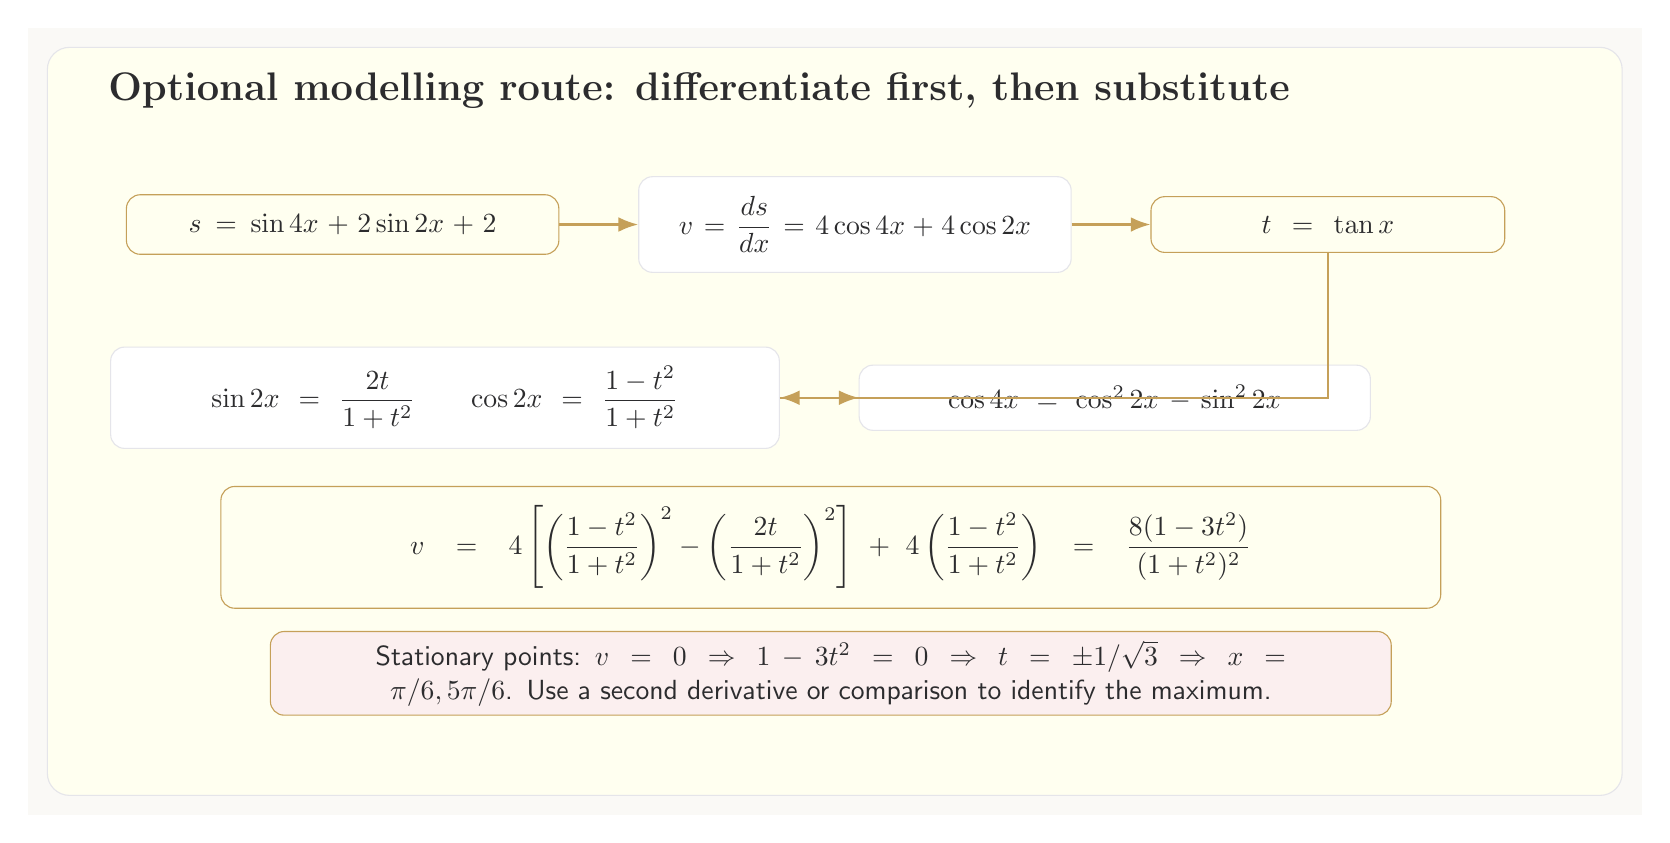
\begin{tikzpicture}[every node/.style={font=\sffamily,text=Text},box/.style={draw=LineSoft,fill=white,rounded corners=5pt,align=center,inner sep=7pt},good/.style={draw=Accent,fill=Ivory,rounded corners=5pt,align=center,inner sep=7pt},arrow/.style={-{Latex[length=2.5mm]},draw=Accent,line width=.8pt}]
\fill[Canvas] (-.5,-.5) rectangle (20,9.5);
\draw[LineSoft,fill=Ivory,rounded corners=8pt] (-.25,-.25) rectangle (19.75,9.25);
\node[anchor=west,font=\bfseries\Large] at (.4,8.7) {Optional modelling route: differentiate first, then substitute};
\node[good,text width=5cm] (s) at (3.5,7) {$s=\sin4x+2\sin2x+2$};
\node[box,text width=5cm,right=1cm of s] (d) {$v=\dfrac{ds}{dx}=4\cos4x+4\cos2x$};
\node[good,text width=4cm,right=1cm of d] (t) {$t=\tan x$};
\draw[arrow] (s)--(d); \draw[arrow] (d)--(t);
\node[box,text width=8cm] (forms) at (4.8,4.8) {$\sin2x=\dfrac{2t}{1+t^2}$\qquad $\cos2x=\dfrac{1-t^2}{1+t^2}$};
\node[box,text width=6cm,right=1cm of forms] (cos4) {$\cos4x=\cos^22x-\sin^22x$};
\draw[arrow] (t.south) |- (forms.east); \draw[arrow] (forms)--(cos4);
\node[good,text width=15cm] at (9.7,2.9) {$\displaystyle v=4\left[\left(\frac{1-t^2}{1+t^2}\right)^2-\left(\frac{2t}{1+t^2}\right)^2\right]+4\left(\frac{1-t^2}{1+t^2}\right)=\frac{8(1-3t^2)}{(1+t^2)^2}$};
\node[draw=Accent,fill=Warning,rounded corners=5pt,text width=14cm,align=center] at (9.7,1.3) {Stationary points: $v=0\Rightarrow 1-3t^2=0\Rightarrow t=\pm 1/\sqrt3\Rightarrow x=\pi/6,5\pi/6$. Use a second derivative or comparison to identify the maximum.};
\end{tikzpicture}
\end{document}
